% Results are based on /private/tmp/evaluation_report_OpenClaw_9Models_LeakFix_Combined_350.xlsx
% and /private/tmp/evaluation_report_5Claws_qwen36flash_cachefix_Cross.xlsx.
% openclaw x GLM 5.1 uses the former for cost/cache accounting; openclaw x Qwen 3.6-flash uses the latter, turns=87.9.

\section{Results}\label{sec:results}

Except for the Lite held-out validation, all main results below report single-run aggregates on the full 350 instances, with worker concurrency fixed at 3. Unlike SWE-bench-style tables that report only resolved rate, we also report \textsc{Total Cost}, mean wall-clock duration, token usage, turn count, and \textsc{Cache Hit Rate}, so coding ability and practical evaluation cost can be interpreted in the same coordinate system. For OpenClaw $\times$ GLM 5.1, we use the cost and cache accounting from the 9-model leak-fix result table; for OpenClaw $\times$ Qwen 3.6-flash, we use the cache-fixed 5-claw cross table and add the mean turn count.

\subsection{The Adapter Makes a General Agent Scorable}\label{sec:adapter_diagnostic}

We first test whether the adapter is merely an engineering wrapper or a necessary condition for OpenClaw to be reliably scored by SWE-bench. Table~\ref{tab:adapter_diagnostic} compares the same GLM 5.1 backbone under the bare adapter and the full adapter. The bare adapter can place OpenClaw in the SWE-bench Docker environment and send the task, but still asks the model to write a unified diff directly in its final response. The full adapter instead lets the model edit repository files through tools and has the runner export the patch from Git state.

\begin{table}[t]
  \centering
  \scriptsize
  \renewcommand{\arraystretch}{1.0}
  \setlength{\tabcolsep}{4pt}
  \caption{Diagnostic comparison between the bare adapter and the full adapter. Both use the same GLM 5.1 backbone and the full-350 workload; the bare adapter is a minimal directly scorable baseline, not a component ablation of the full adapter. \textbf{Apply Failed} is the fraction of instances whose submitted patch cannot be applied to the repository by the SWE-bench evaluator.}
  \label{tab:adapter_diagnostic}
  \begin{tabular*}{0.95\linewidth}{@{\extracolsep{\fill}}lccc@{}}
    \toprule
    \textbf{Configuration} & \textbf{Resolved} & \textbf{Pass@1} & \textbf{Apply Failed} \\
    \midrule
    Bare adapter & 67/350 & 19.1 & 69.1\%\\
    Full adapter & 257/350 & 73.4 & $<1.5\%$ \\
    \bottomrule
  \end{tabular*}
  % \vspace{-3mm}
\end{table}

The results show that minimal access is insufficient to create a reliable SWE-bench evaluation target. The bare adapter reaches only $19.1\%$ resolved rate. The main bottleneck is not that the model cannot edit code at all, but the fragility of directly generating unified-diff text: line numbers, context, hunk headers, or trailing newlines can make the patch fail to apply. The full adapter shifts the output responsibility from ``the model writes patch text'' to ``the model edits repository files and the runner exports the patch,'' reducing apply failures below $1.5\%$ and raising resolved rate to $73.4\%$. The following experiments therefore measure model and claw differences under a unified scoring contract, rather than testing whether a native agent can hand-write a SWE-bench-compatible diff.

\subsection{Variation Along the LLM Axis}\label{sec:variation_llms}

To isolate the contribution of the LLM, we fix OpenClaw as the reference claw and sweep nine models on the full 350-instance set. Table~\ref{tab:a2} reports aggregate results. The highest resolved rate is achieved by GPT 5.5, at $78.0\%$ (273/350), followed by Claude Opus 4.7 at $77.1\%$ (270/350). The lowest cell is Seed 2.0-mini, at $48.6\%$ (170/350). Thus, under the same OpenClaw scaffold, changing only the model produces a $29.4$\,pp Pass@1 spread, confirming that model choice remains a major source of coding-agent performance.

Accuracy ranking, however, is not cost ranking. GPT 5.5 has the highest Pass@1, but its full 350-instance run costs $\$1399.1$; Claude Opus 4.7 is only $0.9$\,pp lower, with cost $\$1082.0$. By contrast, DeepSeek-V4 Pro reaches $71.7\%$ Pass@1 at total cost $\$81.3$, while DeepSeek-V4 Flash reaches $70.3\%$ at only $\$8.2$. Qwen 3.6-flash reaches $66.0\%$ Pass@1 at $\$71.5$; GLM 5.1 reaches $73.4\%$ under cache-fixed cost accounting at $\$277.0$. These results show that cost-aware reporting is not an auxiliary log but a necessary dimension for interpreting benchmark results: similar resolved rates can correspond to evaluation costs that differ by orders of magnitude.

\begin{table}[t]
  \centering
  \scriptsize
  \renewcommand{\arraystretch}{1}
  \setlength{\tabcolsep}{3.3pt}
  \caption{LLM-axis variation: OpenClaw $\times$ 9 models on the full 350-instance Claw-SWE-Bench. Cost is total API cost for the full run (USD); In/Out are total input/output tokens (millions); Turns is average turns; Cache is cache hit rate. Rows are sorted by Pass@1; the best Pass@1 and lowest Cost are in \textbf{bold}.}
  \label{tab:a2}
  \begin{tabular*}{0.95\linewidth}{@{\extracolsep{\fill}}ll|cccccccc@{}}
    \toprule
    \textbf{Model} & \textbf{Type} & \textbf{Resolved} & \textbf{Pass@1} & \textbf{Cost} & \textbf{Dur} & \textbf{In(M)} & \textbf{Out(M)} & \textbf{Turns} & \textbf{Cache} \\
    \midrule
    GPT 5.5             & Flagship & \textbf{273} & \textbf{78.0} & 1399.1 & 603.7 & 40.3 & 15.7 & 67.0 & 97.3 \\
    Claude Opus 4.7     & Flagship & 270 & 77.1 & 1082.0 & 424.6 & 35.6 & 6.2  & 61.6 & 97.0 \\
    GLM 5.1             & Flagship & 257 & 73.4 & 277.0  & 586.8 & 27.6 & 9.3  & 80.6 & 96.5 \\
    DeepSeek-V4 Pro     & Flagship & 251 & 71.7 & 81.3   & 662.3 & 19.3 & 11.0 & 47.1 & 97.4 \\
    Kimi K2.6            & Flagship & 234 & 66.9 & 633.7  & 1235.3& 75.6 & 12.1 & 78.7 & 92.1 \\
    MiniMax M2.7        & Flagship & 215 & 61.4 & 196.7  & 1165.6& 25.0 & 9.0  & 94.8 & 96.2 \\
    \midrule
    DeepSeek-V4 Flash   & Flash    & 246 & 70.3 & \textbf{8.2}   & 430.0 & 13.8 & 12.9 & 51.2 & 98.5 \\
    Qwen 3.6-flash      & Flash    & 231 & 66.0 & 71.5   & 636.0 & 38.9 & 7.5  & 87.9 & 97.6 \\
    Seed 2.0-mini       & Flash    & 170 & 48.6 & 19.4   & 1153.0& 89.8 & 21.6 & 44.4 & 79.4 \\
    \bottomrule
  \end{tabular*}
  % \vspace{-3mm}
\end{table}

Cache hit rate explains some cost differences, but not all of them. DeepSeek-V4 Flash has the highest cache hit rate ($98.5\%$) and the lowest cost. Yet Claude Opus 4.7 and GPT 5.5 also have cache hit rates near $97\%$, while their total costs still exceed $\$1000$. Qwen 3.6-flash has a cache hit rate of $97.6\%$ and costs $\$71.47$; GLM 5.1 costs $\$277.00$ at a $96.5\%$ cache hit rate. Cost is therefore jointly affected by model price, input/output tokens, cache policy, and adapter call path. We report cache hit rate as a diagnostic field for cost accounting, not as a measure of model or harness capability.

\subsection{Effect of Future-Commit Cleanup}\label{sec:leak_fix}

As described in \S\ref{sec:exec_pipeline} and \S\ref{sec:experiments}, the main experiments clean reachable Git history later than \texttt{base\_commit} for non-Python SWE-bench-Multilingual instances. To estimate the effect of this treatment on result accounting, we fix OpenClaw and compare nine models before and after cleanup on the 300 Multilingual instances; adapter, prompt, budget, and evaluator settings are otherwise identical.



Figure~\ref{fig:leak_fix_openclaw} shows that Pass@1 after cleanup is never higher than before cleanup, consistent with the expectation that future-commit visibility can inflate resolved rate. The impact is not uniform: Claude Opus 4.7 drops the most ($84.7\%\rightarrow76.7\%$, $-8.0$\,pp), Kimi 2.6 drops by $5.0$\,pp, and Qwen 3.6-flash drops by $2.0$\,pp; GPT 5.5, MiniMax M2.7, and Seed 2.0-mini change by about $1$\,pp or less. We therefore use cleanup results as the main accounting basis; the before/after comparison is only used to document the necessity and magnitude of the fairness treatment.

\subsection{Variation Along the Claw Axis}\label{sec:variation_harnesses}

To isolate the effect of the claw or harness, we fix the model and sweep the claw axis. Table~\ref{tab:b} reports aggregate results for five claws on GLM 5.1 and Qwen 3.6-flash; the cost and cache fields for OpenClaw $\times$ GLM 5.1 use the same leak-fix accounting as Table~\ref{tab:a2}. On GLM 5.1, OpenClaw achieves the highest Pass@1 ($73.4\%$), followed closely by hermes-agent ($71.1\%$) and zeroclaw ($70.3\%$); the generic baseline has the lowest cost ($\$85.84$) but drops to $63.1\%$ Pass@1. On Qwen 3.6-flash, OpenClaw is again highest ($66.0\%$), with hermes-agent and zeroclaw at $62.6\%$ and $58.3\%$; the generic baseline falls to $38.6\%$.

These results show that the claw is not merely a wrapper. With the same GLM 5.1 model, Pass@1 across the five claws ranges from $60.9\%$ to $73.4\%$, a $12.5$\,pp spread. With the same Qwen 3.6-flash model, the spread is larger, from $38.6\%$ to $66.0\%$, or $27.4$\,pp. In other words, changing only the harness-specific agent loop, tool interface, workspace management, and stopping policy can produce performance differences comparable to, or larger than, neighboring model tiers.
\begin{figure}[t]
  \centering
  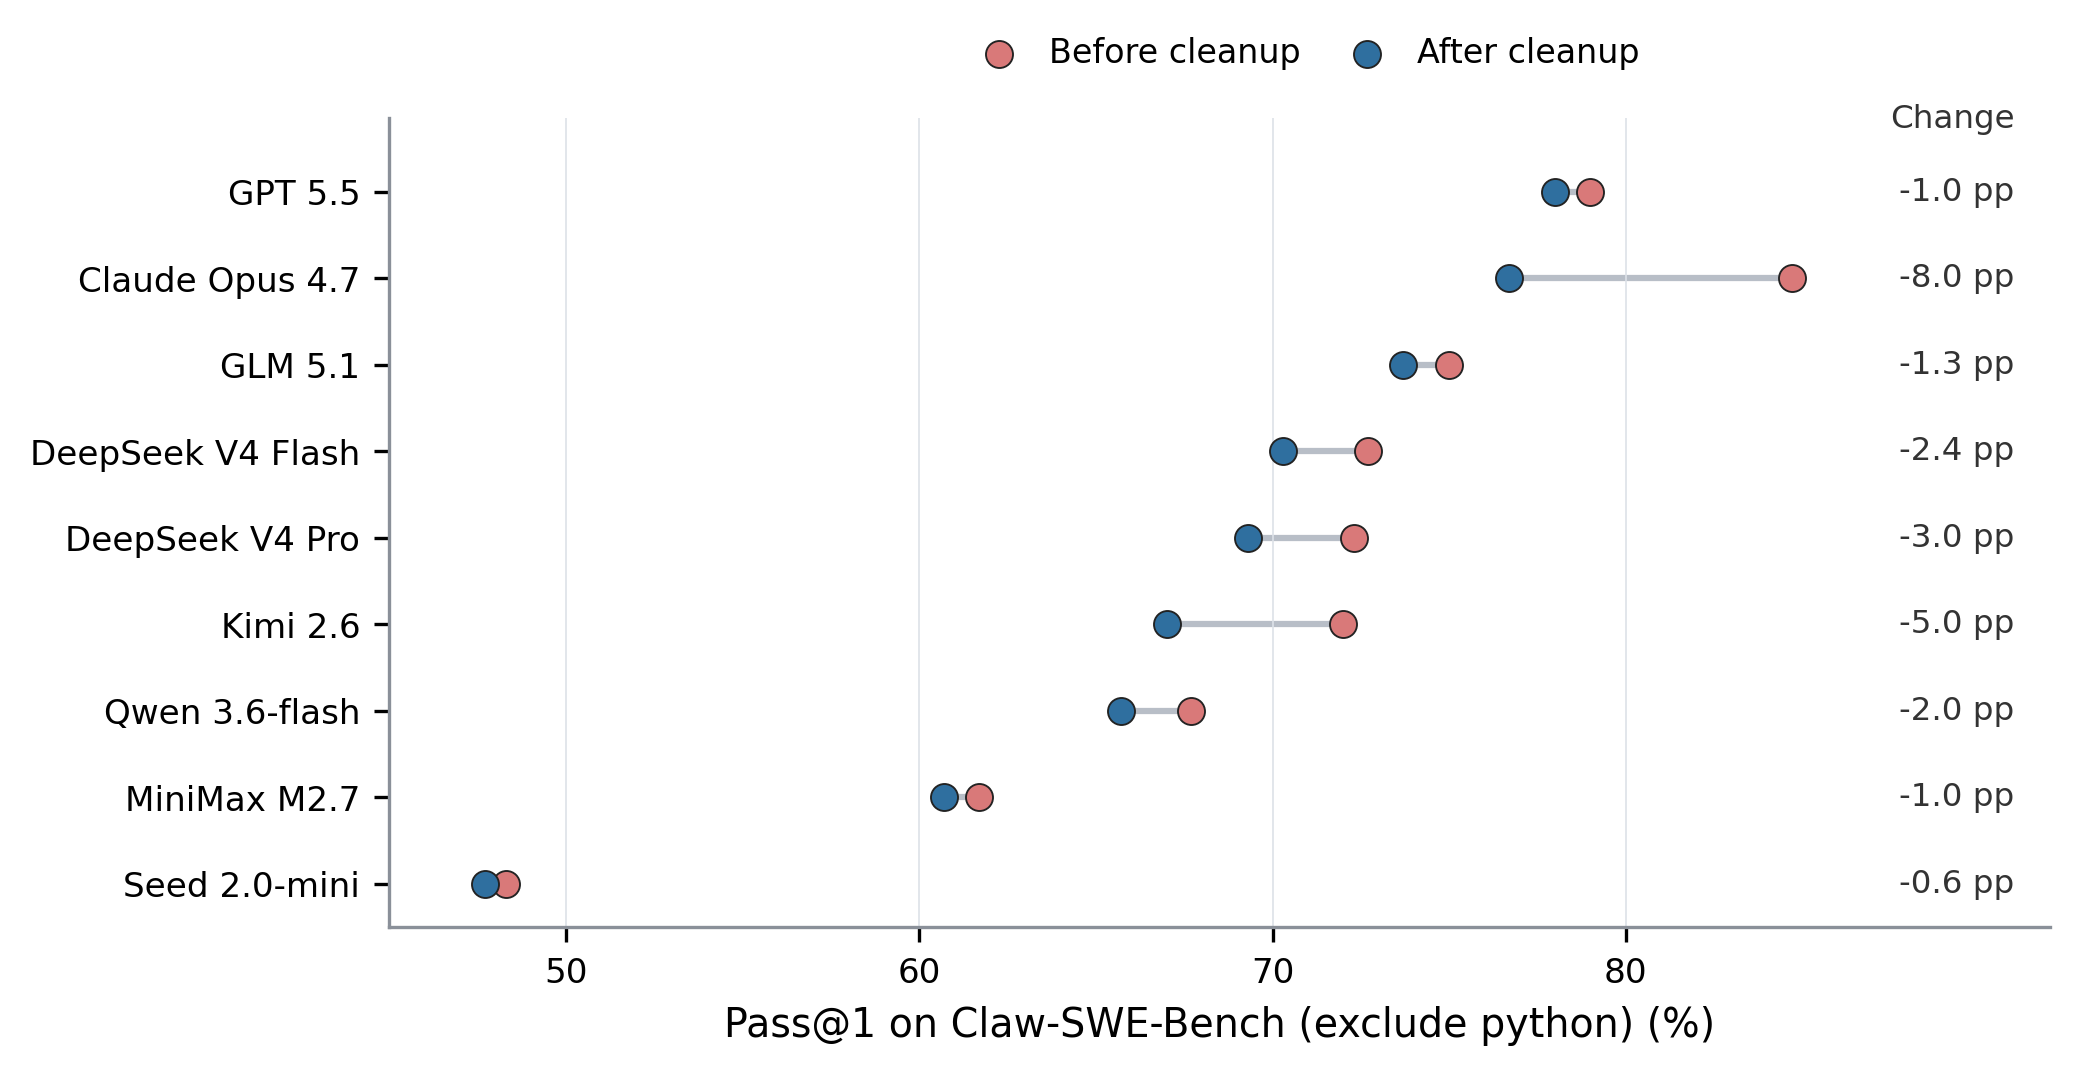
\includegraphics[width=0.9\linewidth]{figs/F_leak_fix_openclaw_multilingual.png}
  \vspace{-2mm}
  \caption{Effect of future-commit cleanup on the OpenClaw model sweep. After cleanup, Pass@1 does not increase for any of the nine models; drops range from $0.6$ to $8.0$\,pp.}
  % \vspace{-4mm}
  \label{fig:leak_fix_openclaw_multilingual}
\end{figure}

\begin{table}[t]
  \centering
  \scriptsize
  \renewcommand{\arraystretch}{1}
  \setlength{\tabcolsep}{3.0pt}
  \caption{Claw-axis variation: five claws $\times$ two models on the full 350-instance Claw-SWE-Bench. Cost is total API cost for the full run (USD); In/Out are total input/output tokens (millions); Cache is cache hit rate. Within each model group, the best Pass@1 and lowest Cost are in \textbf{bold}.}
  \label{tab:b}
  \begin{tabular*}{0.95\linewidth}{@{\extracolsep{\fill}}ll|ccccccc@{}}
    \toprule
    \textbf{Claw} & \textbf{Model} & \textbf{Resolved} & \textbf{Pass@1} & \textbf{Cost} & \textbf{Dur} & \textbf{In(M)} & \textbf{Out(M)} & \textbf{Cache} \\
    \midrule
    openclaw     & GLM 5.1        & \textbf{257} & \textbf{73.4} & 277.0 & 586.8 & 27.6 & 9.3 & 96.5 \\
    hermes-agent & GLM 5.1        & 249 & 71.1 & 330.6 & 675.1 & 93.1 & 5.5 & 91.3 \\
    zeroclaw     & GLM 5.1        & 246 & 70.3 & 383.4 & 538.2 & 989.7 & 4.2 & 90.4 \\
    genericagent      & GLM 5.1        & 221 & 63.1 & \textbf{85.8} & 576.4 & 99.7 & 5.1 & 66.8 \\
    nanobot      & GLM 5.1        & 213 & 60.9 & 768.8 & 1166.3 & 333.9 & 8.5 & 77.2 \\
    \midrule
    openclaw     & Qwen 3.6-flash & \textbf{231} & \textbf{66.0} & 71.5 & 636.0 & 38.9 & 7.5 & 97.6 \\
    hermes-agent & Qwen 3.6-flash & 219 & 62.6 & 103.3 & 638.6 & 44.3 & 7.2 & 97.4 \\
    zeroclaw     & Qwen 3.6-flash & 204 & 58.3 & 49.3 & 428.9 & 1057.9 & 6.1 & 96.9 \\
    genericagent      & Qwen 3.6-flash & 135 & 38.6 & \textbf{14.5} & 321.4 & 103.1 & 2.8 & 74.7 \\
    nanobot      & Qwen 3.6-flash & 166 & 47.4 & 133.1 & 562.7 & 418.8 & 8.2 & 63.9 \\
    
    \bottomrule
  \end{tabular*}
  % \vspace{-4mm}
\end{table}

\paragraph{Cost--accuracy analysis of Figure~\ref{fig:pareto_frontier}.}
Cost further changes how claw rankings should be interpreted. Figure~\ref{fig:pareto_frontier} is a two-dimensional projection of Table~\ref{tab:b}: for each claw--model combination, the horizontal axis uses the full 350-instance \textsc{Total Cost}, and the vertical axis uses Pass@1 from the same row; OpenClaw $\times$ GLM 5.1 follows the leak-fix cost accounting in Table~\ref{tab:a2}. The Pareto frontier consists of points that are not dominated by another combination with both lower cost and higher Pass@1.

In this plane, the lowest-cost endpoint is generic $\times$ Qwen 3.6-flash ($\$14.50$, $38.6\%$), but its resolved rate is low. Zeroclaw $\times$ Qwen 3.6-flash increases cost to $\$49.26$ and raises Pass@1 to $58.3\%$; OpenClaw $\times$ Qwen 3.6-flash reaches $66.0\%$ at $\$71.47$. In the GLM 5.1 group, OpenClaw is the high-accuracy endpoint with $73.4\%$ Pass@1 at $\$277.00$; hermes-agent and zeroclaw have similar resolved rates, but are dominated by OpenClaw $\times$ GLM 5.1 because they are both more expensive and less accurate. This result shows that claw comparison cannot be read only as a within-model resolved-rate ranking. A cross-model, cross-claw, cost-aware Pareto view is needed to distinguish genuinely useful operating points from systems that only look close on one axis.

% \subsection{Held-Out Validation of Lite-80}\label{sec:lite_heldout}

% Section~\ref{sec:lite} validates Lite-80 on calibration columns for aggregate parity and ranking stability. For a low-cost subset to be useful as an evaluation entry point, it should also be checked on a new system not used during calibration. We therefore use \textsc{OpenSQuILLA} as a held-out validation system and compare its \textsc{Pass@1} on full-350 and Lite-80. This experiment does not reselect Lite instances and does not enter the Lite construction objective; it only tests whether a new general-purpose agent has similar resolved rate on the two evaluation surfaces.

% Table~\ref{tab:lite_heldout_opensquilla} gives the reporting format. The final result will list resolved count and \textsc{Pass@1} on both full-350 and Lite-80, together with the percentage-point gap defined as Lite-80 rate minus full-350 rate. If the gap remains small, Lite-80 is not merely fitted to the calibration pool; it also approximates the full benchmark's aggregate evaluation effect on a new general-purpose agent.

% \begin{table}[t]
%   \centering
%   \scriptsize
%   \renewcommand{\arraystretch}{0.95}
%   \setlength{\tabcolsep}{4pt}
%   \caption{Lite-80 held-out validation on \textsc{OpenSQuILLA}. \textsc{OpenSQuILLA} is not used in Lite construction or calibration; $\Delta$ is Lite-80 \textsc{Pass@1} minus full-350 \textsc{Pass@1}, in percentage points.}
%   \label{tab:lite_heldout_opensquilla}
%   \begin{tabular*}{\linewidth}{@{\extracolsep{\fill}}lcccc@{}}
%     \toprule
%     \textbf{System} & \textbf{Full-350} & \textbf{Lite-80} & \textbf{$\Delta$} & \textbf{Scale} \\
%     \midrule
%     \textsc{OpenSQuILLA} & --/350 (--\%) & --/80 (--\%) & -- pp & 22.9\% \\
%     \bottomrule
%   \end{tabular*}
%   \vspace{-3mm}
% \end{table}

\subsection{Interpreting Cache and Cost}\label{sec:cost_perf}

Cache hit rate varies substantially across claws. For example, under GLM 5.1, the cache hit rates of OpenClaw, hermes-agent, and zeroclaw are $96.5\%$, $91.3\%$, and $90.4\%$, respectively, while generic is $66.8\%$. Under Qwen 3.6-flash, OpenClaw, hermes-agent, and zeroclaw are all near $97\%$, but nanobot is $63.9\%$ and generic is $74.7\%$. These differences indicate that adapter behavior and provider-side caching can substantially affect the actual API bill. We therefore list cache hit rate in all main result tables so that readers can determine whether cost differences come from model price, token usage, or cache reuse.

At the same time, cache hit rate should not be over-interpreted. A higher cache hit rate does not necessarily imply higher Pass@1 or a stronger harness; it is first a run-level and billing-level diagnostic. Our conclusions therefore use a two-layer reading: Pass@1 measures the final coding outcome, cost measures the resources required to complete the same evaluation, and cache hit rate explains one important mechanism in cost accounting. Together, these quantities form a repeatable, comparable, and scorable SWE-style coding-agent benchmark.
